
\section*{CHƯƠNG 1. TỔNG QUAN HỆ THỐNG}
\setcounter{section}{1}
\setcounter{subsection}{0} %LƯU Ý MỖI LẦN THÊM CHƯƠNG MỚI CẦN THÊM CÂU NÀY ĐỂ RESET THỨ TỰ CỦA SUBSECTON VỀ 1
\setcounter{table}{0} % LƯU Ý SAU MỖI LẦN GỌI BẢNG HAY HÌNH ẢNH PHẢI THÊM CÂU NÀY ĐỂ RESET THỨ TỰ
\setcounter{figure}{0} %% LƯU Ý SAU MỖI LẦN GỌI BẢNG HAY HÌNH ẢNH PHẢI THÊM CÂU NÀY ĐỂ RESET THỨ TỰ
\addcontentsline{toc}{section}
% \addcontentsline{toc}{section}
{\numberline{}CHƯƠNG 1. TỔNG QUAN HỆ THỐNG}
Trong chương này, chúng em sẽ tiến hành phân tích hệ thống cho dự án đề tài "Hệ thống quản lý ECG" dựa trên các mục tiêu
đã nêu ra trong Mục Đề xuất hệ thống ở Phần mở đầu. Trước tiên bài toán đặt ra ở hệ thống phần mềm điện tim là có thể có:

- Một thiết bị để có thể giúp mẹ bầu đo được những thông tin cần thiết.

- Trực quan và tiêu chuẩn hoá những thông tin đo được
bằng hình ảnh hoặc số liệu để bác sĩ có thể dựa vào đó để đưa ra những đánh giá cho mẹ bầu. Ngoài ra những thông tin này
có thể hữu ích trong việc theo dõi sức khỏe tim mạch, theo dõi hiệu quả của liệu pháp 
và hỗ trợ quyết định của người dùng.

- Quản trị viên sẽ là người có thể phân công bác sĩ để chăm sóc, theo dõi sức khoẻ từ
xa cho mẹ bầu. 

Chi tiết về việc phân tích các yêu cầu hệ thống sẽ được chúng em trình bày ở các chương dưới.


\subsection{Yêu cầu hệ thống}
\subsubsection{Yêu cầu về người dùng hệ thống}
Hệ thống được thiết kế để phục vụ các đối tượng sau:
\begin{itemize}
    \item Bệnh nhân: Người sử dụng hệ thống để thực hiện kiểm tra ECG thông qua Bluetooth và theo dõi sức khỏe của mình. Bệnh nhân có quyền truy cập vào kết quả ECG của mình, được một bác sĩ theo dõi và có thể theo dõi các thông tin liên quan đến điện tim và sức khoẻ.
    \item Bác sĩ: Người sử dụng hệ thống để xem và đánh giá kết quả ECG của bệnh nhân, đưa ra nhận xét và đề xuất điều trị. Bác sĩ có thể trao đổi với bệnh nhân và gửi thông báo quan trọng liên quan đến chăm sóc sức khỏe.
    \item Quản trị viên: Người sử dụng hệ thống để quản lý các tài khoản người dùng, phân công bệnh nhân cho bác sĩ và quản lý mối quan hệ giữa bác sĩ và bệnh nhân.
\end{itemize}

\subsubsection{Yêu cầu chức năng}
Các chức năng chính của hệ thống bao gồm: 
\begin{adjustwidth}{2em}{}
  \begin{itemize}
      \item Ghi lại dữ liệu điện tim: Hệ thống cho phép ghi lại tín hiệu điện tim từ máy đo ECG (Electrocardiogram) hay thiết bị đo điện tim khác. Dữ liệu được chuyển tới ứng dụng của người dùng thông qua Bluetooth để lưu trữ, phân tích và có thể xem lại sau này.
  
      \item Hiển thị và phân tích dữ liệu: Hệ thống hiển thị dữ liệu điện tim theo dạng đồ thị. Hệ thống cũng hỗ trợ xuất ra các tệp đã được chuẩn hoá cho các dữ liệu chuỗi thời gian (time-series database) để phục vụ mục đích phân tích và nghiên cứu sâu hơn.
  
      \item Lưu trữ: Hệ thống hỗ trợ lưu dữ liệu mà người dùng đo được từ thiết bị trên cả ứng dụng và trên server của hệ thống. Dữ liệu điện tim cũng được đồng bộ hóa và lưu trữ trên máy chủ của hệ thống. Qua quá trình đồng bộ hóa, dữ liệu từ ứng dụng được truyền đến máy chủ và được lưu trữ an toàn và bảo mật trên hệ thống. Việc lưu trữ dữ liệu điện tim trên cả ứng dụng và máy chủ giúp đảm bảo rằng dữ liệu quan trọng này được lưu trữ một cách đáng tin cậy và có sẵn cho phân tích hoặc sử dụng tương lai.
  
      \item Trao đổi và chia sẻ thông tin về dữ liệu điện tim: Hệ thống giúp người dùng có thể trao đổi trực tiếp với nhau, chia sẻ kết quả đo điện tim, hỏi đáp về các vấn đề sức khỏe hoặc thảo luận về các quyết định. Điều này mang lại sự tiện lợi và hỗ trợ đáng kể cho người dùng trong việc xác định về tình trạng sức khoẻ hiện tại của bản thân.
  \end{itemize}
  \end{adjustwidth}
  
  

  
  
Hệ thống hỗ trợ các chức năng cơ bản sau đối với người dùng:

\textbf{Đối với người dùng là bệnh nhân:}
\begin{itemize}
    \item Đăng nhập và đăng ký tài khoản bằng thông tin cá nhân, bao gồm tên, địa chỉ email, ngày sinh, số điện thoại và mật khẩu.
    \item Cập nhật các thông tin cá nhân.
    \item Xem kết quả ECG của mình, bao gồm biểu đồ và các thông số liên quan.
    \item Theo dõi các tin tức liên quan đến sức khoẻ và tim mạch.
    \item Nhận thông báo và có thể trao đổi trực tiếp với bác sĩ về tình hình sức khoẻ và các kết quả đo được từ thiết bị.
\end{itemize}

Đối với người dùng là bác sĩ:

\begin{itemize}
    \item Được cấp tài khoản để sử dụng hệ thống.
    \item Cập nhật các thông tin cá nhân.
    \item Xem danh sách bệnh nhân được phân công cho mình và xem kết quả ECG của từng bệnh nhân.
    \item Đánh giá và đưa ra nhận xét về kết quả ECG của bệnh nhân.
    \item Trao đổi các thông tin liên quan đến tình hình sức khoẻ và kết quả đo của bệnh nhân.
\end{itemize}

Đối với người dùng là quản trị viên:
\begin{itemize}
    \item Đăng nhập và đăng ký tài khoản bằng thông tin cá nhân, bao gồm tên, địa chỉ email, số điện thoại và mật khẩu.
    \item Cập nhật thông tin cá nhân.
    \item Quản lý danh sách người dùng trong hệ thống, bao gồm bệnh nhân và bác sĩ.
    \item Phân công bệnh nhân cho các bác sĩ và quản lý mối quan hệ giữa bác sĩ và bệnh nhân.
    \item Quản lý các tin tức được đăng trên ứng dụng của người dùng.
\end{itemize}

\subsubsection{Yêu cầu phi chức năng}
\begin{itemize}
    \item Hệ thống hỗ trợ ngôn ngữ Tiếng Việt và Tiếng Anh.
    \item Hệ thống có thể tương thích với các loại thiết bị phổ biến hiện nay (với Android: Android 10+, IOS: IOS > 12.1)
    \item Hệ thống đảm bảo tính bảo mật và quyền riêng tư thông tin của người dùng.
    \item Hệ thống phải có giao diện người dùng thân thiện, dễ sử dụng để có thể tương tác mà không gặp quá nhiều khó khăn.
    \item Thời gian phản hồi của hệ thống phải nhanh chóng và ổn định.
    % \item Hệ thống cần sao lưu dữ liệu định kỳ để đảm bảo tính an toàn và khả năng khôi phục dữ liệu khi cần thiết.
\end{itemize}

Thông qua việc phân tích yêu cầu hệ thống, chúng ta có cái nhìn tổng quan về các chức năng, yêu cầu phi chức năng và 
các đối tượng người dùng mà hệ thống phải hỗ trợ. Phần phân tích này sẽ cung cấp cơ sở cho việc thiết kế và phát triển hệ thống quản lý ECG, 
đáp ứng đầy đủ các yêu cầu của người dùng và đảm bảo hiệu suất, bảo mật và tính khả dụng của hệ thống.
\subsection{Phân tích tổng quan hệ thống}

\subsection{Sơ đồ use case}
\subsubsection{Use case tổng quát hệ thống}
Dựa vào những phân tích về yêu cầu chức năng, các use case trong hệ thống được chúng em thể hiện ở hình dưới 
  \begin{figure}[H]
    \centering
    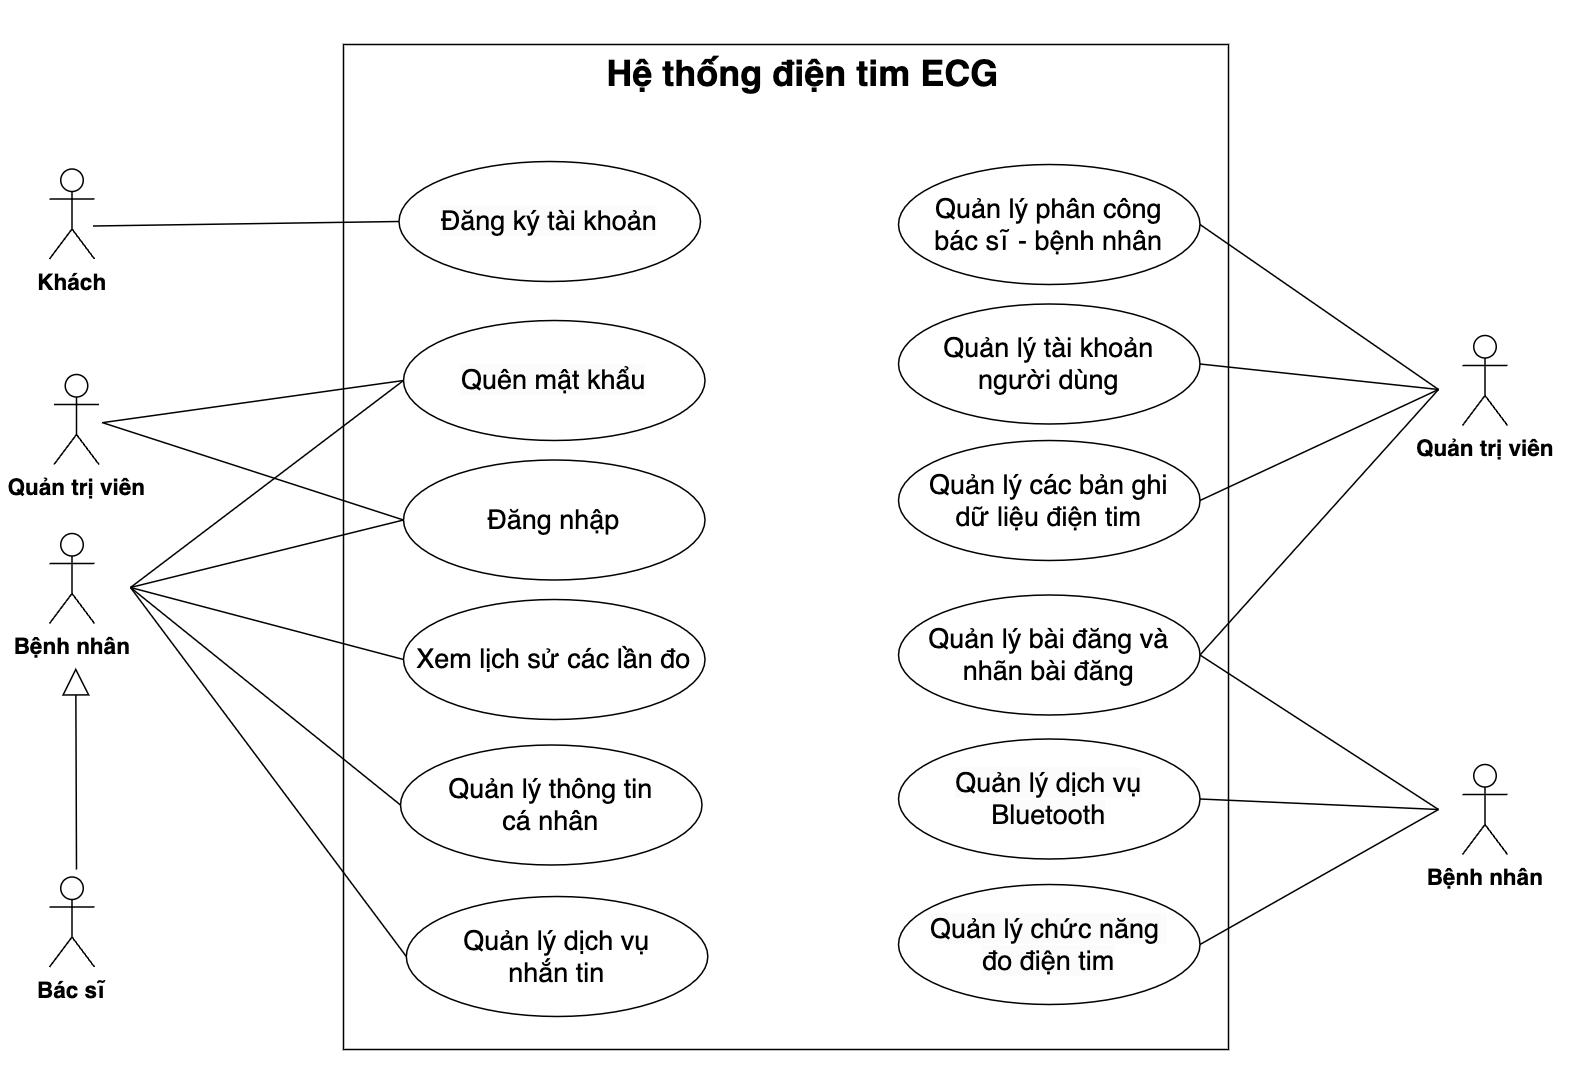
\includegraphics[width=17cm,height=14cm]{Images/use_case/use_case_general.png}
    \caption[Sơ đồ use case tổng quát của hệ thống]{\bfseries \fontsize{12pt}{0pt}
    \selectfont Sơ đồ use case tổng quát của hệ thống}
    \label{use_case_general} %đặt tên cho ảnh
  \end{figure}

\subsubsection{Use case chức năng đăng ký tài khoản}
  \begin{figure}[H]
    \centering
    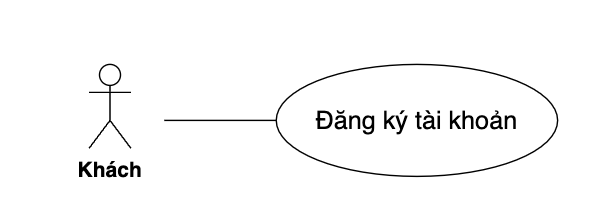
\includegraphics[width=15cm,height=6cm]{Images/use_case/use_case_register.png}
    \caption[Sơ đồ use case chức năng đăng ký tài khoản]{\bfseries \fontsize{12pt}{0pt}
    \selectfont Sơ đồ use case chức năng đăng ký tài khoản}
    \label{use_case_register} %đặt tên cho ảnh
  \end{figure}

  \begin{table}[H]
    \caption{\bfseries \fontsize{12pt}{0pt}\selectfont Bảng phân tích use case chức năng đăng ký}
    \centering
    \begin{tabularx}{0.9\textwidth}{|c|X|}
      \hline
      \textbf{Tên chức năng} & \textbf{Đăng ký} \\
      \hline
      Tác nhân & Khách \\
      \hline
      Mô tả & Cho phép người dùng đăng ký tài khoản để truy cập vào App/Web 
      và truy cập các tài nguyên của hệ thống \\
      \hline
      Điều kiện trước & Người dùng cần có kết nối Internet \\
      \hline
      Dòng sự kiện chính & 
      % \begin{tabular}{@{}l@{}}
        Chi tiết luồng sự kiện được thể hiện ở Hình \ref{register} và Hình\\
      % \end{tabular} \\
      \hline
    \end{tabularx}
  \end{table}

\subsubsection{Use case chức năng quên mật khẩu}
  \begin{figure}[H]
    \centering
    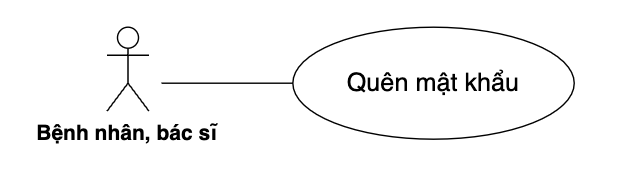
\includegraphics[width=15cm,height=6cm]{Images/use_case/use_case_forgot_password.png}
    \caption[Sơ đồ use case chức năng quên mật khẩu]{\bfseries \fontsize{12pt}{0pt}
    \selectfont Sơ đồ use case chức năng quên mật khẩu}
    \label{use_case_forgot_password} %đặt tên cho ảnh
  \end{figure}

  \begin{table}[H]
    \caption{\bfseries \fontsize{12pt}{0pt}\selectfont Bảng phân tích use case chức năng quên mật khẩu}
    \centering
    \begin{tabularx}{0.9\textwidth}{|c|X|}
      \hline
      \textbf{Tên chức năng} & \textbf{Quên mật khẩu} \\
      \hline
      Tác nhân & Bệnh nhân, Bác sĩ, Quản trị viên \\
      \hline
      Mô tả & Cho phép người dùng lấy lại mật khẩu bằng email khi quên mật khẩu \\
      \hline
      Điều kiện trước & Người dùng cần có kết nối Internet và truy cập được vào email đăng ký \\
      \hline
      Dòng sự kiện chính & 
      % \begin{tabular}{@{}l@{}}
        Chi tiết luồng sự kiện được thể hiện ở Hình \ref{forgot_password} và Hình\\
      % \end{tabular} \\
      \hline
    \end{tabularx}
  \end{table}

\subsubsection{Use case chức năng đăng nhập}
  \begin{figure}[H]
    \centering
    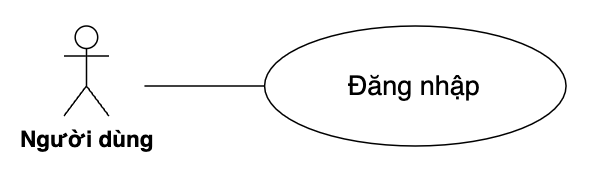
\includegraphics[width=15cm,height=6cm]{Images/use_case/use_case_login.png}
    \caption[Sơ đồ use case chức năng đăng nhập]{\bfseries \fontsize{12pt}{0pt}
    \selectfont Sơ đồ use case chức năng đăng nhập}
    \label{use_case_login} %đặt tên cho ảnh
  \end{figure}

  \begin{table}[H]
    \caption{\bfseries \fontsize{12pt}{0pt}\selectfont Bảng phân tích use case chức năng đăng nhập}
    \centering
    \begin{tabularx}{0.9\textwidth}{|c|X|}
      \hline
      \textbf{Tên chức năng} & \textbf{Đăng nhập} \\
      \hline
      Tác nhân & Bệnh nhân, Bác sĩ, Quản trị viên \\
      \hline
      Mô tả & Cho phép người dùng sử dụng tài khoản để truy cập vào App/Web để truy cập các tài nguyên của hệ thống \\
      \hline
      Điều kiện trước & Người dùng cần có kết nối Internet \\
      \hline
      Dòng sự kiện chính & 
      % \begin{tabular}{@{}l@{}}
        Chi tiết luồng sự kiện được thể hiện ở Hình \ref{login} và Hình\\
      % \end{tabular} \\
      \hline
    \end{tabularx}
  \end{table}

\subsubsection{Use case chức năng xem lịch sử các lần đo}
  \begin{figure}[H]
    \centering
    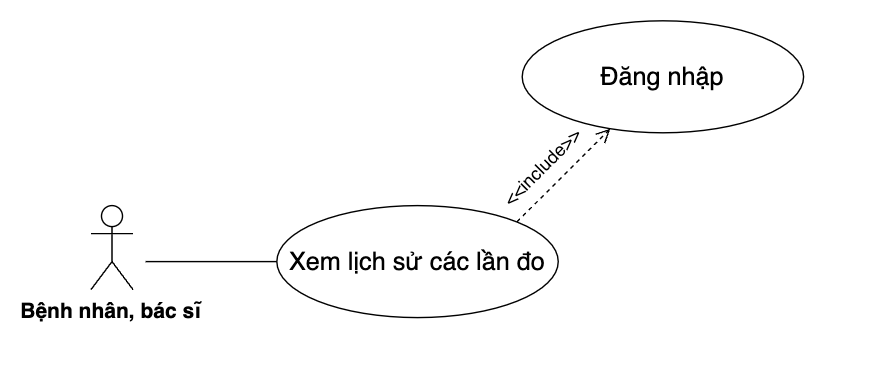
\includegraphics[width=15cm,height=6cm]{Images/use_case/use_case_view_history_record.png}
    \caption[Sơ đồ use case chức năng xem lịch sử các lần đo]{\bfseries \fontsize{12pt}{0pt}
    \selectfont Sơ đồ use case chức năng xem lịch sử các lần đo}
    \label{use_case_view_history_record} %đặt tên cho ảnh
  \end{figure}

  \begin{table}[H]
    \caption{\bfseries \fontsize{12pt}{0pt}\selectfont Bảng phân tích use case chức năng xem lịch sử các lần đo}
    \centering
    \begin{tabularx}{0.9\textwidth}{|c|X|}
      \hline
      \textbf{Tên chức năng} & \textbf{Xem lịch sử các lần đo} \\
      \hline
      Tác nhân & Bệnh nhân, Bác sĩ \\
      \hline
      Mô tả & Cho phép bệnh nhân xem lịch sử các lần đo điện tim và bác sĩ xem được lịch sử các lần đo của bệnh nhân
      mà mình quản lý \\
      \hline
      Điều kiện trước & Người dùng cần có kết nối Internet và đã đăng nhập \\
      \hline
      Dòng sự kiện chính & 
      % \begin{tabular}{@{}l@{}}
        Chi tiết luồng sự kiện được thể hiện ở Hình \ref{view_record_timeline} và Hình\\
      % \end{tabular} \\
      \hline
    \end{tabularx}
  \end{table}

\subsubsection{Use case chức năng quản lý thông tin cá nhân}
  \begin{figure}[H]
    \centering
    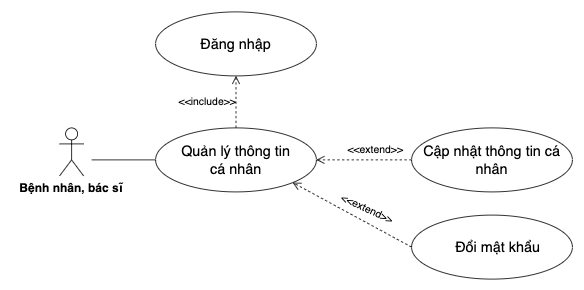
\includegraphics[width=15cm,height=6cm]{Images/use_case/use_case_manage_info.png}
    \caption[Sơ đồ use case chức năng quản lý thông tin cá nhân]{\bfseries \fontsize{12pt}{0pt}
    \selectfont Sơ đồ use case chức năng quản lý thông tin cá nhân}
    \label{use_case_manage_info} %đặt tên cho ảnh
  \end{figure}

  \begin{table}[H]
    \caption{\bfseries \fontsize{12pt}{0pt}\selectfont Bảng phân tích use case chức năng quản lý thông tin cá nhân}
    \centering
    \begin{tabularx}{0.9\textwidth}{|c|X|}
      \hline
      \textbf{Tên chức năng} & \textbf{Quản lý thông tin cá nhân} \\
      \hline
      Tác nhân & Bệnh nhân, Bác sĩ, Quản trị viên \\
      \hline
      Mô tả & Cho phép người dùng thay đổi thông tin cá nhân như số điện thoại, tên hiển thị, mật khẩu \\
      \hline
      Điều kiện trước & Người dùng cần có kết nối Internet và đã đăng nhập \\
      \hline
      Dòng sự kiện chính & 
      % \begin{tabular}{@{}l@{}}
        Chi tiết luồng sự kiện được thể hiện ở Hình \ref{change_user_information}, Hình \ref{change_password} 
        và Hình\\
      % \end{tabular} \\
      \hline
    \end{tabularx}
  \end{table}

\subsubsection{Use case chức năng quản lý dịch vụ nhắn tin}
  \begin{figure}[H]
    \centering
    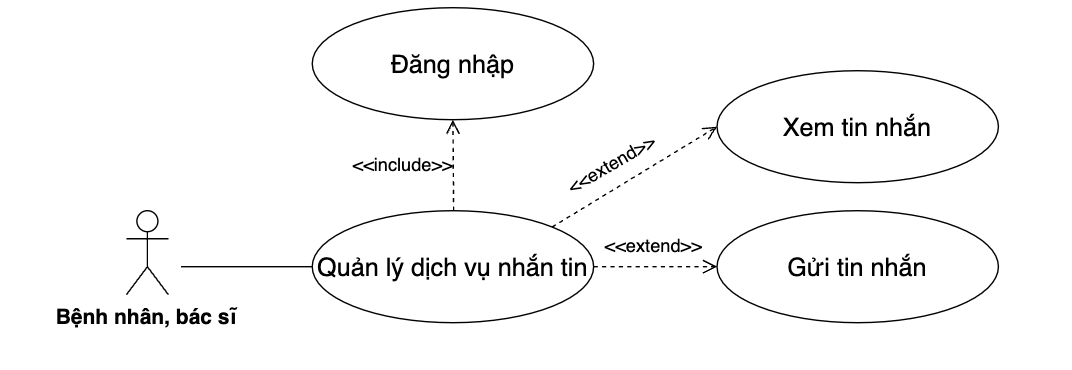
\includegraphics[width=15cm,height=6cm]{Images/use_case/use_case_send_receive_message.png}
    \caption[Sơ đồ use case chức năng quản lý dịch vụ nhắn tin]{\bfseries \fontsize{12pt}{0pt}
    \selectfont Sơ đồ use case chức năng quản lý dịch vụ nhắn tin}
    \label{use_case_send_receive_message} %đặt tên cho ảnh
  \end{figure}

  \begin{table}[H]
    \caption{\bfseries \fontsize{12pt}{0pt}\selectfont Bảng phân tích use case chức năng quản lý dịch vụ nhắn tin}
    \centering
    \begin{tabularx}{0.9\textwidth}{|c|X|}
      \hline
      \textbf{Tên chức năng} & \textbf{Quản lý dịch vụ nhắn tin} \\
      \hline
      Tác nhân & Bệnh nhân, Bác sĩ \\
      \hline
      Mô tả & Cho phép người dùng sử dụng tài khoản để nhắn tin trao đổi, tin nhắn sau khi được gửi sẽ được
      hiện ở dưới cùng trong khung chat \\
      \hline
      Điều kiện trước & Người dùng cần có kết nối Internet, đã đăng nhập và đã được phân công trong bảng bệnh nhân - bác sĩ \\
      \hline
      Dòng sự kiện chính & 
      % \begin{tabular}{@{}l@{}}
        Chi tiết luồng sự kiện được thể hiện ở Hình \ref{send_and_receive_message} và Hình\\
      % \end{tabular} \\
      \hline
    \end{tabularx}
  \end{table}

\subsubsection{Use case chức năng quản lý đo điện tim}
  \begin{figure}[H]
    \centering
    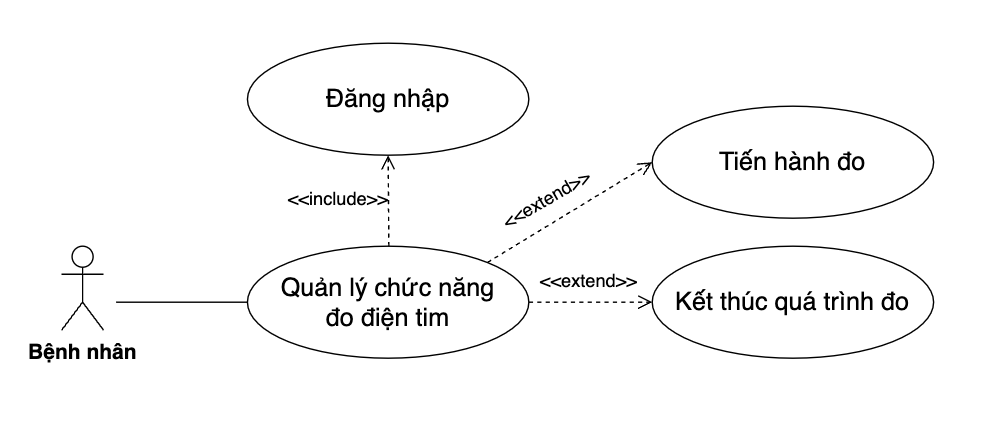
\includegraphics[width=15cm,height=6cm]{Images/use_case/use_case_measure_ecg.png}
    \caption[Sơ đồ use case chức năng quản lý đo điện tim]{\bfseries \fontsize{12pt}{0pt}
    \selectfont Sơ đồ use case chức năng quản lý đo điện tim}
    \label{use_case_measure_ecg} %đặt tên cho ảnh
  \end{figure}

  \begin{table}[H]
    \caption{\bfseries \fontsize{12pt}{0pt}\selectfont Bảng phân tích use case chức năng quản lý đo điện tim}
    \centering
    \begin{tabularx}{0.9\textwidth}{|c|X|}
      \hline
      \textbf{Tên chức năng} & \textbf{Quản lý đo điện tim} \\
      \hline
      Tác nhân & Bệnh nhân \\
      \hline
      Mô tả & Cho phép người dùng thực hiện thao tác bắt đầu/ kết thúc quá trình đo của mình. \\
      \hline
      Điều kiện trước & Người dùng cần bật Bluetooth và đã kết nối với thiết bị đo điện tim \\
      \hline
      Dòng sự kiện chính & 
      % \begin{tabular}{@{}l@{}}
        Chi tiết luồng sự kiện được thể hiện ở Hình \ref{start_measuring_ecg} và Hình \ref{end_measuring_ecg} \\
      % \end{tabular} \\
      \hline
    \end{tabularx}
  \end{table}

\subsubsection{Use case chức năng quản lý dịch vụ Bluetooth}
  \begin{figure}[H]
    \centering
    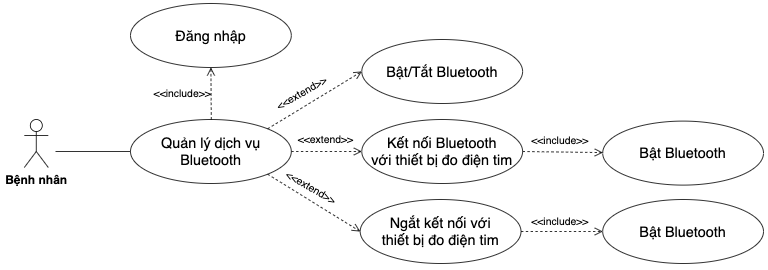
\includegraphics[width=15cm,height=6cm]{Images/use_case/use_case_bluetooth.png}
    \caption[Sơ đồ use case chức năng quản lý dịch vụ Bluetooth]{\bfseries \fontsize{12pt}{0pt}
    \selectfont Sơ đồ use case chức năng quản lý dịch vụ Bluetooth}
    \label{use_case_bluetooth} %đặt tên cho ảnh
  \end{figure}

  \begin{table}[H]
    \caption{\bfseries \fontsize{12pt}{0pt}\selectfont Bảng phân tích use case chức năng quản lý dịch vụ Bluetooth}
    \centering
    \begin{tabularx}{0.9\textwidth}{|c|X|}
      \hline
      \textbf{Tên chức năng} & \textbf{Quản lý dịch vụ Bluetooth} \\
      \hline
      Tác nhân & Bệnh nhân \\
      \hline
      Mô tả & Cho phép người dùng thực hiện các thao tác liên quan đến việc bật tắt và quản lý kết nối với thiết bị điện tim \\
      \hline
      Điều kiện trước & Điện thoại của người dùng có hỗ trợ Bluetooth \\
      \hline
      Dòng sự kiện chính & 
      % \begin{tabular}{@{}l@{}}
        Chi tiết luồng sự kiện được thể hiện ở Hình \ref{} và Hình\\
      % \end{tabular} \\
      \hline
    \end{tabularx}
  \end{table}

\subsubsection{Use case chức năng quản lý bài đăng và nhãn bài đăng}
  \begin{figure}[H]
    \centering
    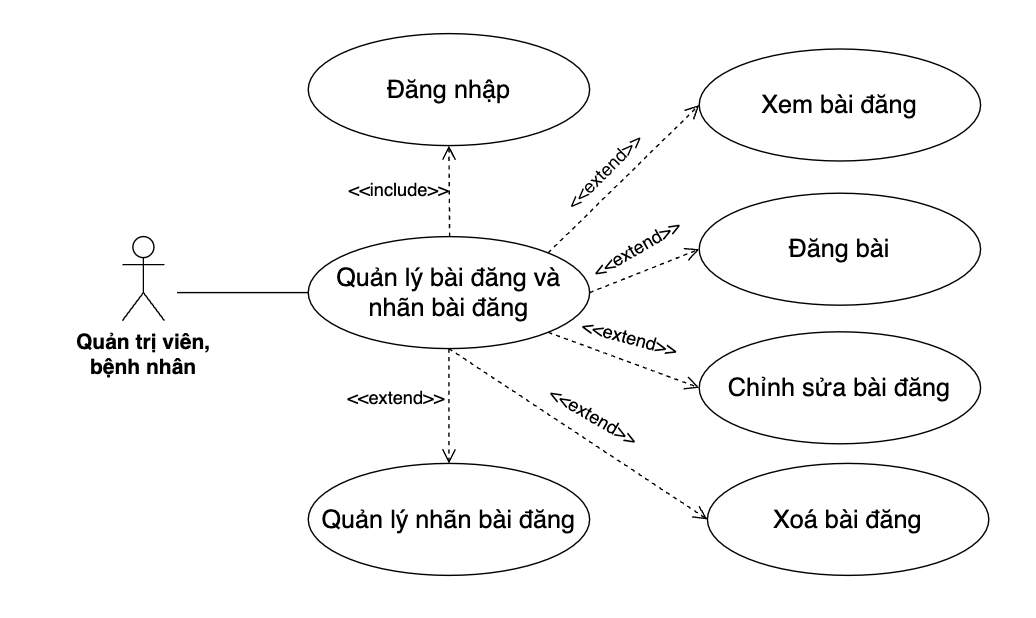
\includegraphics[width=15cm,height=8cm]{Images/use_case/use_case_news.png}
    \caption[Sơ đồ use case chức năng quản lý bài đăng]{\bfseries \fontsize{12pt}{0pt}
    \selectfont Sơ đồ use case chức năng quản lý bài đăng}
    \label{use_case_news} %đặt tên cho ảnh
  \end{figure}

  \begin{table}[H]
    \caption{\bfseries \fontsize{12pt}{0pt}\selectfont Bảng phân tích use case chức năng quản lý bài đăng và nhãn bài đăng}
    \centering
    \begin{tabularx}{0.9\textwidth}{|c|X|}
      \hline
      \textbf{Tên chức năng} & \textbf{quản lý bài đăng và nhãn bài đăng} \\
      \hline
      Tác nhân & Bệnh nhân, Quản trị viên \\
      \hline
      Mô tả & Cho phép bệnh nhân xem các bài đăng xem các thông tin liên quan đến sức khoẻ, trong đó quản trị viên có thể
      xem, thêm, sửa, xoá các bài đăng đó  \\
      \hline
      Điều kiện trước & Người dùng cần có kết nối Internet và đã đăng nhập \\
      \hline
      Dòng sự kiện chính & 
      % \begin{tabular}{@{}l@{}}
        Chi tiết luồng sự kiện được thể hiện ở Hình \ref{view_news} và Hình\\
      % \end{tabular} \\
      \hline
    \end{tabularx}
  \end{table}

  \begin{figure}[H]
    \centering
    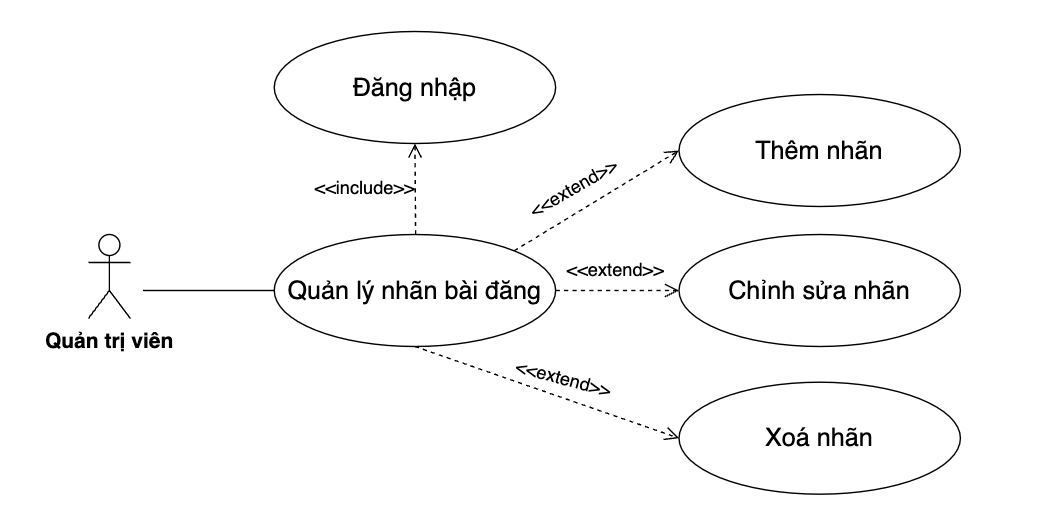
\includegraphics[width=15cm,height=7cm]{Images/use_case/use_case_category_news.png}
    \caption[Sơ đồ use case chức năng quản lý nhãn bài đăng]{\bfseries \fontsize{12pt}{0pt}
    \selectfont Sơ đồ use case chức năng quản lý nhãn bài đăng}
    \label{use_case_category_news} %đặt tên cho ảnh
  \end{figure}

  \begin{table}[H]
    \caption{\bfseries \fontsize{12pt}{0pt}\selectfont Bảng phân tích use case chức năng quản lý nhãn bài đăng}
    \centering
    \begin{tabularx}{0.9\textwidth}{|c|X|}
      \hline
      \textbf{Tên chức năng} & \textbf{Quản lý nhãn bài đăng} \\
      \hline
      Tác nhân & Quản trị viên \\
      \hline
      Mô tả & Cho phép quản trị viên thêm, sửa, xoá nhãn bài đăng và kết hợp nhãn cho từng bài đăng \\
      \hline
      Điều kiện trước & Người dùng cần có kết nối Internet và đã đăng nhập với tư cách là quản trị viên \\
      \hline
      Dòng sự kiện chính & 
      % \begin{tabular}{@{}l@{}}
        Chi tiết luồng sự kiện được thể hiện ở Hình\\
      % \end{tabular} \\
      \hline
    \end{tabularx}
  \end{table}

\subsubsection{Use case chức năng quản lý các bản ghi dữ liệu điện tim}
  \begin{figure}[H]
    \centering
    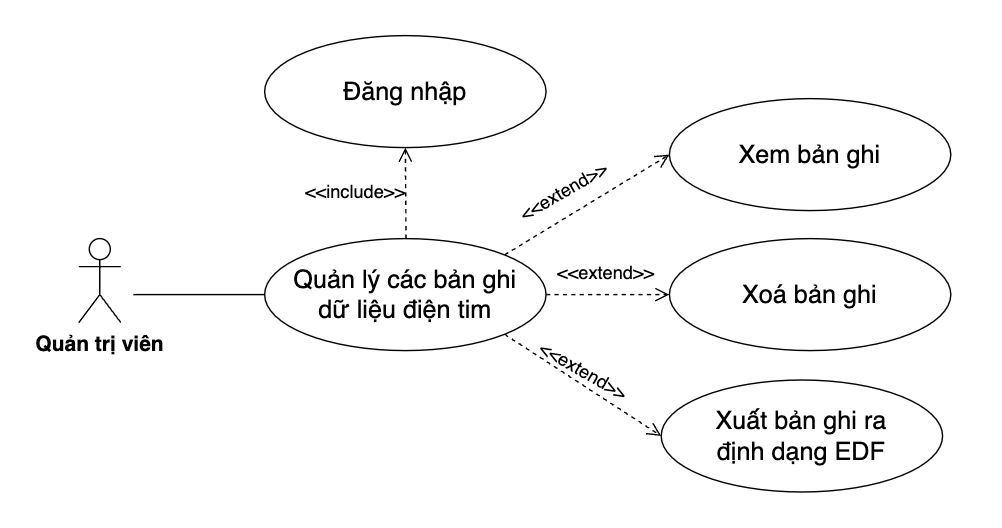
\includegraphics[width=15cm,height=7cm]{Images/use_case/use_case_manage_records.png}
    \caption[Sơ đồ use case chức năng quản lý các bản ghi dữ liệu điện tim]{\bfseries \fontsize{12pt}{0pt}
    \selectfont Sơ đồ use case chức năng quản lý các bản ghi dữ liệu điện tim}
    \label{use_case_manage_records} %đặt tên cho ảnh
  \end{figure}

  \begin{table}[H]
    \caption{\bfseries \fontsize{12pt}{0pt}\selectfont Bảng phân tích use case chức năng quản lý các bản ghi dữ liệu điện tim}
    \centering
    \begin{tabularx}{0.9\textwidth}{|c|X|}
      \hline
      \textbf{Tên chức năng} & \textbf{Quản lý các bản ghi dữ liệu điện tim} \\
      \hline
      Tác nhân & Quản trị viên \\
      \hline
      Mô tả & Cho phép quản trị viên quản lý  những bản ghi và xuất ra những định dạng phục vụ cho việc chẩn đoán của bác sĩ \\
      \hline
      Điều kiện trước & Người dùng cần có kết nối Internet và đã đăng nhập với tư cách là quản trị viên \\
      \hline
      Dòng sự kiện chính & 
      % \begin{tabular}{@{}l@{}}
        Chi tiết luồng sự kiện được thể hiện ở Hình\\
      % \end{tabular} \\
      \hline
    \end{tabularx}
  \end{table}

\subsubsection{Use case chức năng quản lý tài khoản người dùng}
  \begin{figure}[H]
    \centering
    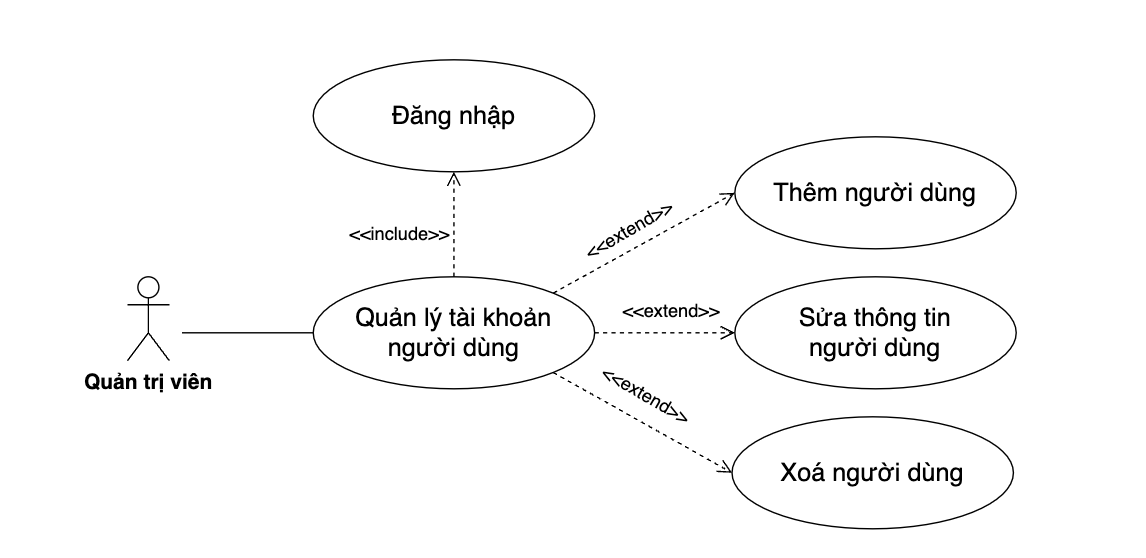
\includegraphics[width=15cm,height=7cm]{Images/use_case/use_case_manage_users.png}
    \caption[Sơ đồ use case chức năng quản lý tài khoản người dùng]{\bfseries \fontsize{12pt}{0pt}
    \selectfont Sơ đồ use case chức năng quản lý tài khoản người dùng}
    \label{use_case_manage_users} %đặt tên cho ảnh
  \end{figure}

  \begin{table}[H]
    \caption{\bfseries \fontsize{12pt}{0pt}\selectfont Bảng phân tích use case chức năng quản lý tài khoản người dùng}
    \centering
    \begin{tabularx}{0.9\textwidth}{|c|X|}
      \hline
      \textbf{Tên chức năng} & \textbf{Quản lý tài khoản người dùng} \\
      \hline
      Tác nhân & Quản trị viên \\
      \hline
      Mô tả & Cho phép quản trị viên thực hiện các hành động thêm, sửa, xoá, tìm kiến đối với tài khoản người dùng \\
      \hline
      Điều kiện trước & Người dùng cần có kết nối Internet và đã đăng nhập với tư cách là quản trị viên \\
      \hline
      Dòng sự kiện chính & 
      % \begin{tabular}{@{}l@{}}
        Chi tiết luồng sự kiện được thể hiện ở Hình \ref{} và Hình\\
      % \end{tabular} \\
      \hline
    \end{tabularx}
  \end{table}

\subsubsection{Use case chức năng quản lý phân công bác sĩ - bệnh nhân}
  \begin{figure}[H]
    \centering
    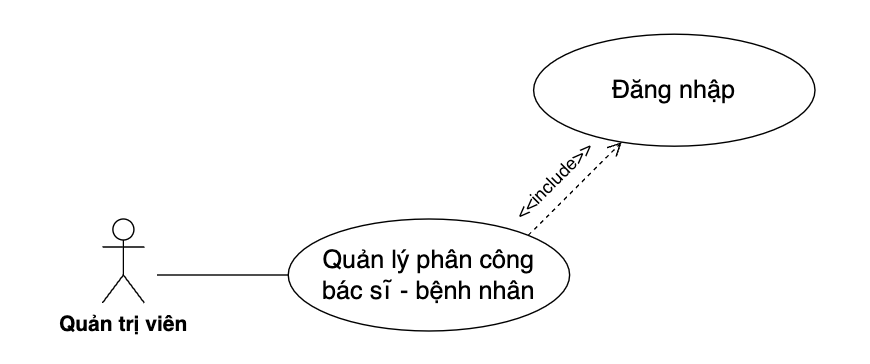
\includegraphics[width=15cm,height=6cm]{Images/use_case/use_case_assign_doctor.png}
    \caption[Sơ đồ use case chức năng quản lý phân công bác sĩ - bệnh nhân]{\bfseries \fontsize{12pt}{0pt}
    \selectfont Sơ đồ use case chức năng quản lý phân công bác sĩ - bệnh nhân}
    \label{use_case_assign_doctor} %đặt tên cho ảnh
  \end{figure}

  \begin{table}[H]
    \caption{\bfseries \fontsize{12pt}{0pt}\selectfont Bảng phân tích use case chức năng quản lý phân công bác sĩ - bệnh nhân}
    \centering
    \begin{tabularx}{0.9\textwidth}{|c|X|}
      \hline
      \textbf{Tên chức năng} & \textbf{quản lý phân công bác sĩ - bệnh nhân} \\
      \hline
      Tác nhân & Quản trị viên \\
      \hline
      Mô tả & Cho phép quản trị viên phân công bác sĩ chăm sóc, theo dõi với từng bệnh nhân tương ứng để có thể xem bản ghi
      và trao đổi về sức khoẻ \\
      \hline
      Điều kiện trước & Người dùng cần có kết nối Internet và đã đăng nhập với tư cách là quản trị viên \\
      \hline
      Dòng sự kiện chính & 
      % \begin{tabular}{@{}l@{}}
        Chi tiết luồng sự kiện được thể hiện ở Hình \ref{} và Hình\\
      % \end{tabular} \\
      \hline
    \end{tabularx}
  \end{table}


\subsubsection{Sơ đồ kiến trúc hệ thống}
Hệ thống chúng em xây dựng được chia làm ba phần Device, Application và Server. Cụ thể: 
\begin{itemize}
  \item Device: Thiết bị phần cứng đo điện tim, để kết nối với App bệnh nhân thông qua Bluetooth 
  \item Application: Bao gồm ứng dụng của bệnh nhân, ứng dụng của bác sĩ và Website của Admin
  \item Server: Bao gồm các Services để xử lý các yêu cầu gửi từ Application, cơ sở dữ liệu và Cloud lưu trữ
\end{itemize}
 
Trong hệ thống thì Devices là phần mà chúng em sẽ không trực tiếp thực hiện trong đồ án này, Application và Server sẽ là
phần mà đồ án chúng em thực hiện. Ở trong sơ đồ kiến trúc hệ thống riêng có bệnh nhân sẽ có tương tác trực tiếp với Devices,
còn lại khối Application sẽ tương tác với Server thông qua API với giao thức HTTP. Khi nhận được yêu cầu từ Application,
Server sẽ thực hiện xử lý dữ liệu và gửi lại thông tin mà Application yêu cầu.

\begin{figure}[H]
  \centering
  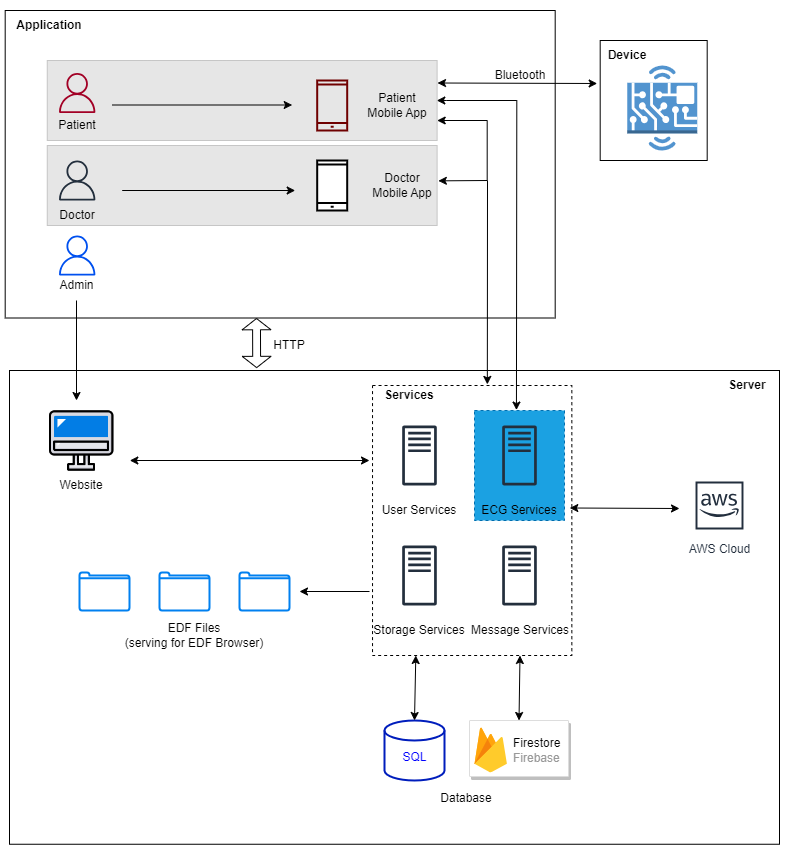
\includegraphics[width=16cm,height=18cm]{Images/system/fmECG_architecture-System Architecture.drawio.png}
  \caption[Kiến trúc tổng quan hệ thống]{\bfseries \fontsize{12pt}{0pt}\selectfont Kiến trúc tổng quan hệ thống}
  \label{fmECG_architecture-System} %đặt tên cho ảnh
\end{figure}

\subsubsection{Sơ đồ khối phần mềm}

\paragraph{Ứng dụng di động cho bệnh nhân}
\mbox{}

\begin{figure}[H]
  \centering
  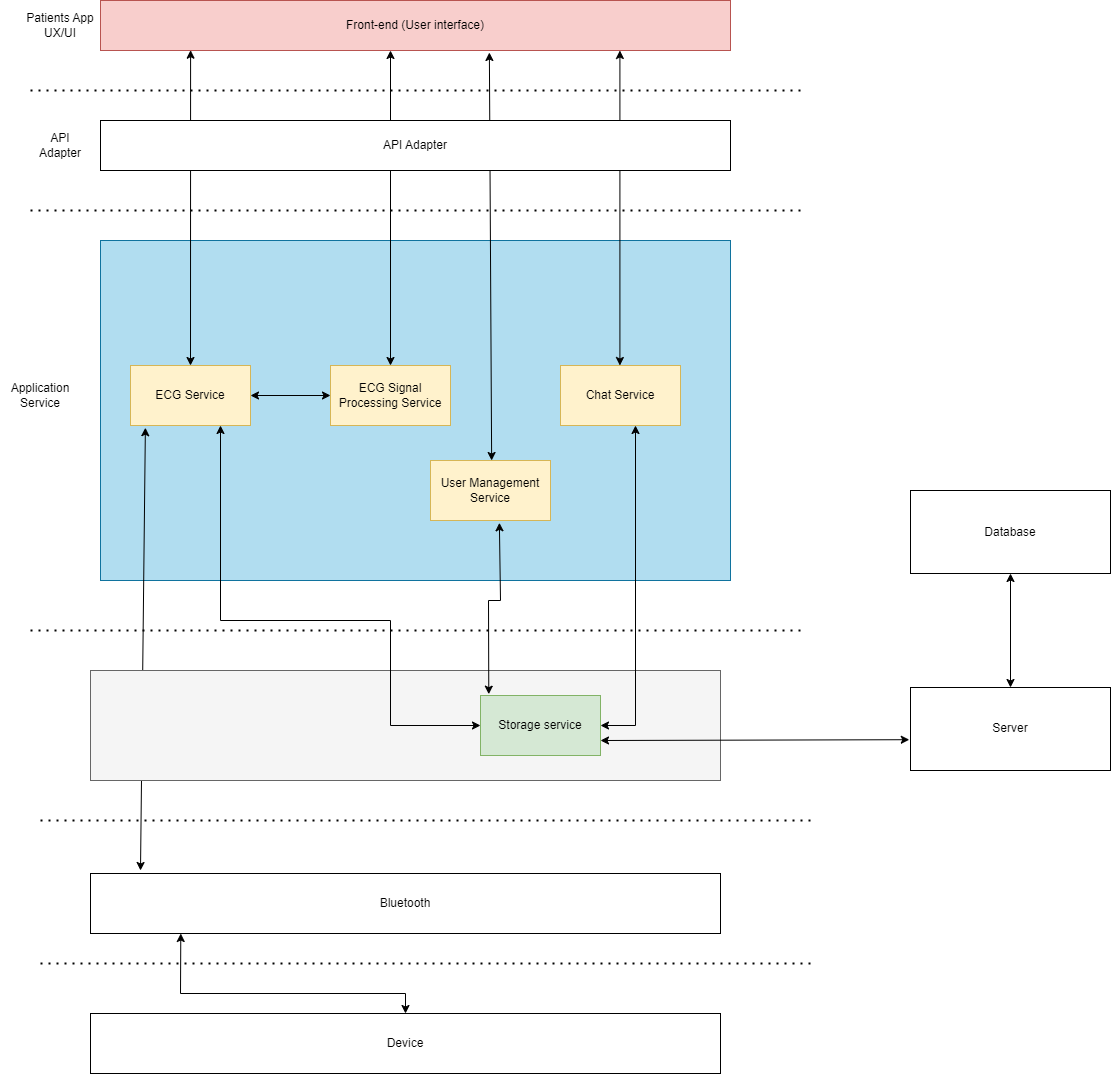
\includegraphics[width=16cm,height=18cm]{Images/system/fmECG_architecture-Patient.drawio.png}
  \caption[Sơ đồ khối cho App bệnh nhân]{\bfseries \fontsize{12pt}{0pt}\selectfont Sơ đồ khối cho App bệnh nhân}
  \label{fmECG_architecture-Patient} %đặt tên cho ảnh
\end{figure}

Trong hình trên, lớp trên cùng User interface là lớp để người dùng tương tác và thực hiện lời gọi thông qua API Adapter, 
các yêu cầu của người dùng sẽ được xử lý thông qua Services và phản hồi lại với người dùng qua giao diện. Dưới đây là phần
giải thích Services trong hình:

\begin{itemize}
  \item ECG Service: Khối có nhiệm vụ xử lý yêu cầu cho các trạng thái đo: thực hiện đo, kết thúc đo, lưu kết quả đo
  \item ECG Signal Processing Service: Khối có nhiệm vụ xử lý tín hiệu đo để phân tích sâu, hiển thị lên màn hình
  \item User Management Service: Khối có nhiệm vụ xử lý các vấn đề liên quan đến người dùng như đăng nhập, đăng ký
  \item Chat Service: Khối có nhiệm vụ quản lý việc chat, trao đổi thông tin
  \item Storage Service: Khối có nhiệm vụ lưu thông tin vào bộ nhớ
\end{itemize}

Riêng với App cho bệnh nhân thì sẽ có Khối Bluetooth và Khối Device để phục vụ cho việc đo điện tim.
\paragraph{Ứng dụng di động cho bác sĩ}
\mbox{}

\begin{figure}[H]
  \centering
  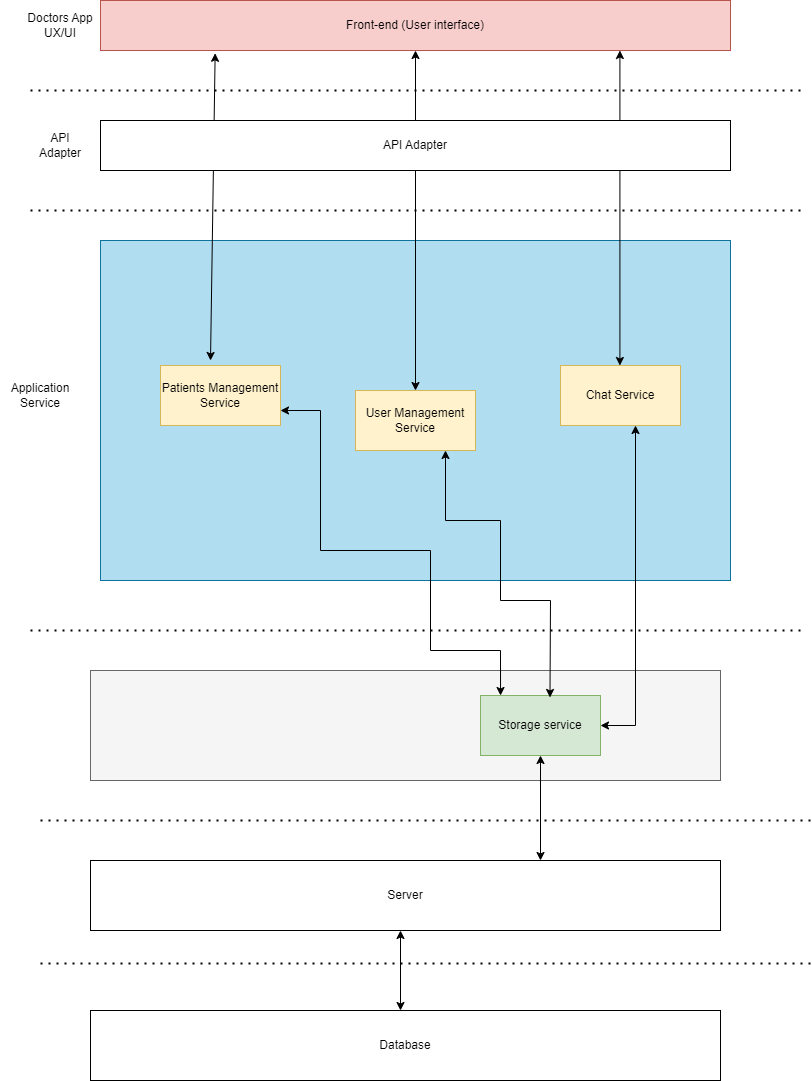
\includegraphics[width=16cm,height=18cm]{Images/system/fmECG_architecture-Doctors.drawio.png}
  \caption[Sơ đồ khói cho App bác sĩ]{\bfseries \fontsize{12pt}{0pt}\selectfont Sơ đồ khối cho App bác sĩ}
  \label{fmECG_architecture-Doctors} %đặt tên cho ảnh
\end{figure}

Về cơ bản, ứng dụng di động cho bác sĩ có những khối tương tự với bệnh nhân, trừ việc bác sĩ sẽ không có hai khối Device
và Bluetooth để phục vụ việc đo như bệnh nhân.


\paragraph{Website cho quản trị viên}
\mbox{}

\begin{figure}[H]
  \centering
  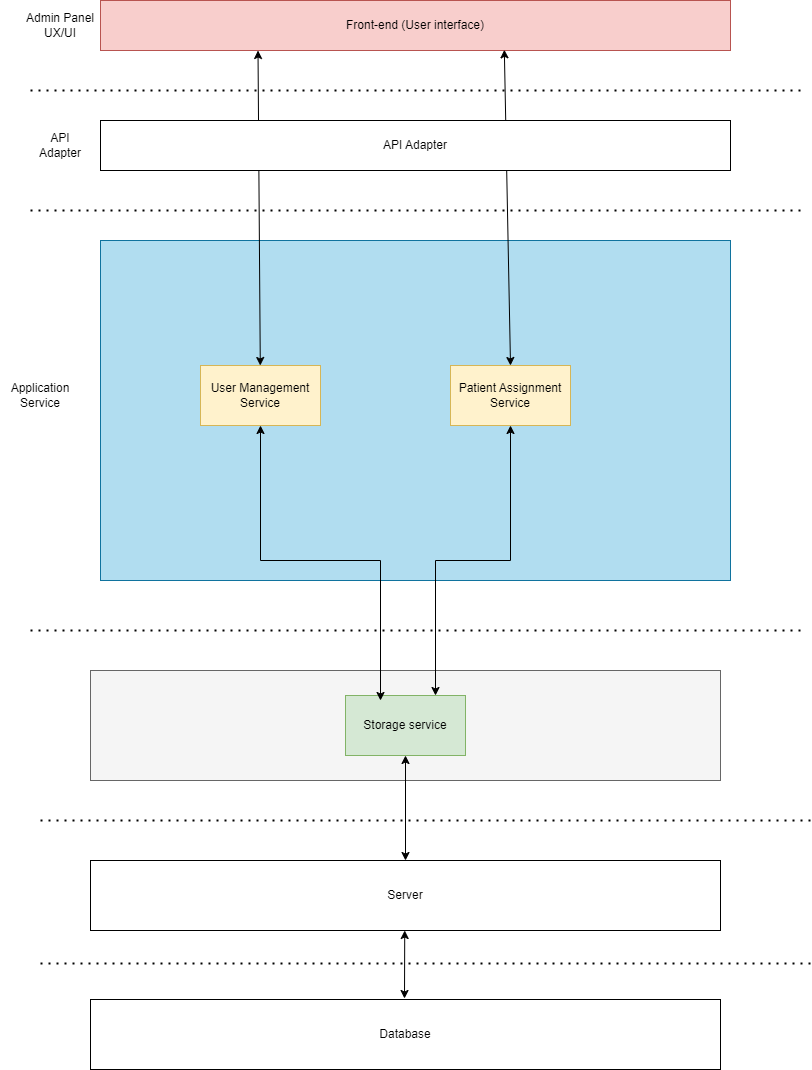
\includegraphics[width=16cm,height=18cm]{Images/system/fmECG_architecture-Admin.drawio.png}
  \caption[Sơ đồ khối cho Website quản trị viên]{\bfseries \fontsize{12pt}{0pt}\selectfont Sơ đồ khối cho Website quản trị viên}
  \label{fmECG_architecture-Admin} %đặt tên cho ảnh
\end{figure}

Quản trị viên sẽ quản lý 2 Services chính đó là quản lý người dùng (User Management Service) và quản lý phân công
bác sĩ - bệnh nhân (Patient Assignment Service), logic và thứ tự các khối tương đồng với ứng dụng dành cho bác sĩ.

Tiếp theo để phân tích cụ thể hơn từng luồng trong hệ thống qua use case, chúng em xin phép được trình bày các sơ đồ tuần
tự. 
\newpage
\subsubsection{Sơ đồ tuần tự}

\paragraph{Sơ đồ tuần tự chức năng đăng ký}
\mbox{}
  \begin{figure}[H]
        \centering
        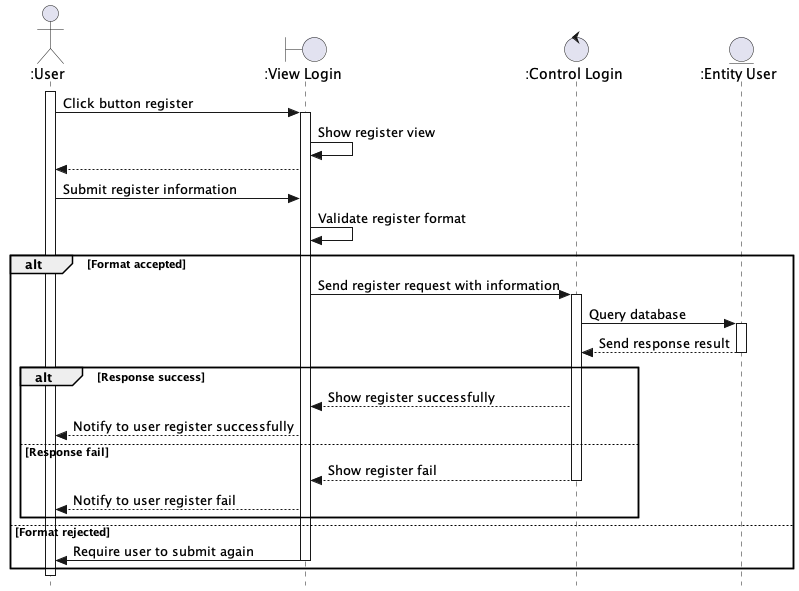
\includegraphics[width=16cm,height=12cm]{Images/mobile_app/register.png}
        \caption[Sơ đồ tuần tự chức năng đăng ký trên App]{\bfseries \fontsize{12pt}{0pt}
        \selectfont Sơ đồ tuần tự chức năng đăng ký trên App}
        \label{register} %đặt tên cho ảnh
  \end{figure}
  Sơ đồ tuần tự trên mô tả chi tiết quá trình người dùng đăng ký vào hệ thống. Người dùng gửi yêu cầu đăng ký, yêu cầu sẽ
  được xử lý bởi Control, nếu có lỗi phát sinh sẽ trả ra lỗi cho người dùng và yêu cầu người dùng nhập lại. Control
  sẽ xử lý cụ thể như thế nào được chúng em thể hiện trong Hình \ref{} trong chương sau.
\paragraph{Sơ đồ tuần tự chức năng đăng nhập}
\mbox{}

    \begin{figure}[H]
         \centering
         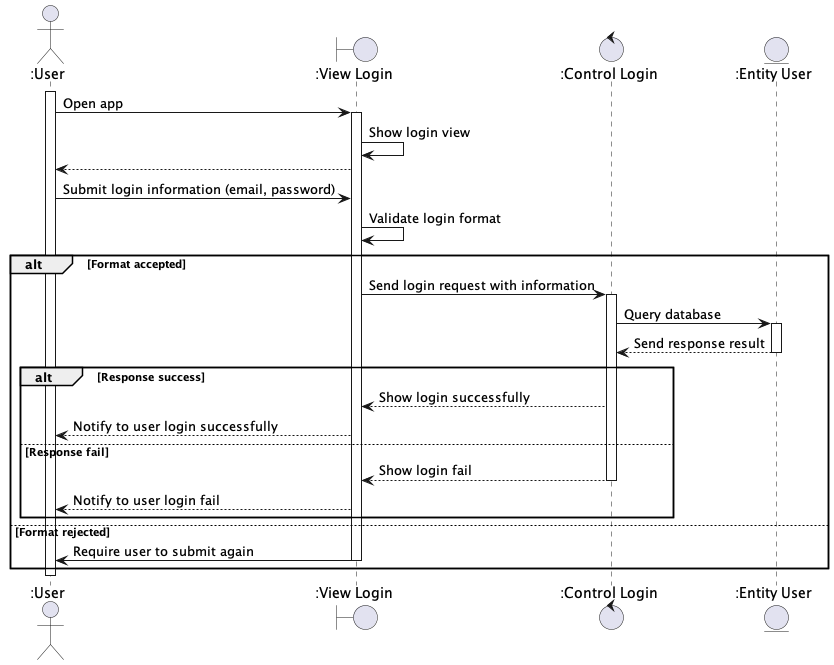
\includegraphics[width=16cm,height=12cm]{Images/mobile_app/login.png}
         \caption[Sơ đồ tuần tự chức năng đăng nhập trên App]{\bfseries \fontsize{12pt}{0pt}
         \selectfont Sơ đồ tuần tự chức năng đăng nhập trên App}
         \label{login} %đặt tên cho ảnh
    \end{figure}

  Sơ đồ tuần tự trên mô tả chi tiết quá trình người dùng đăng nhập vào hệ thống. Người dùng gửi yêu cầu đăng nhập, yêu cầu sẽ
  được xử lý bởi Control, nếu có lỗi phát sinh sẽ trả ra lỗi cho người dùng và yêu cầu người dùng nhập lại. Việc Control
  sẽ xử lý cụ thể yêu cầu người dùng được chúng em thể hiện trong Hình \ref{} trong chương sau.

\paragraph{Sơ đồ tuần tự chức năng quên mật khẩu}
\mbox{}

  \begin{figure}[H]
        \centering
        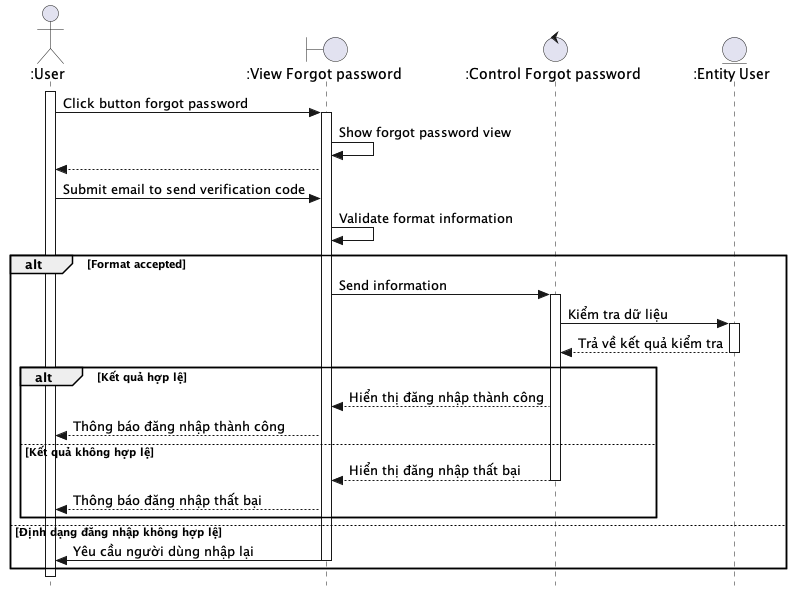
\includegraphics[width=16cm,height=12cm]{Images/mobile_app/forgot_password.png}
        \caption[Sơ đồ tuần tự chức năng quên mật khẩu trên App]{\bfseries \fontsize{12pt}{0pt}
        \selectfont Sơ đồ tuần tự chức năng quên mật khẩu trên App}
        \label{forgot_password} %đặt tên cho ảnh
  \end{figure}

    Sơ đồ tuần tự trên mô tả chi tiết quá trình người dùng lấy lại mật khẩu. Người dùng nhập email đã đăng ký tài khoản,
  và gửi yêu cầu lấy lại mật khẩu, Control xử lý gửi đến email một mã xác thực, người dùng nhập đúng mã xác thực sẽ được thay
  đổi mật khẩu mới. Control xử lý cụ thể yêu cầu được chúng em thể hiện trong Hình \ref{} trong chương sau.

\paragraph{Sơ đồ tuần tự chức năng xem lịch sử các lần đo}
\mbox{}

    \begin{figure}[H]
         \centering
         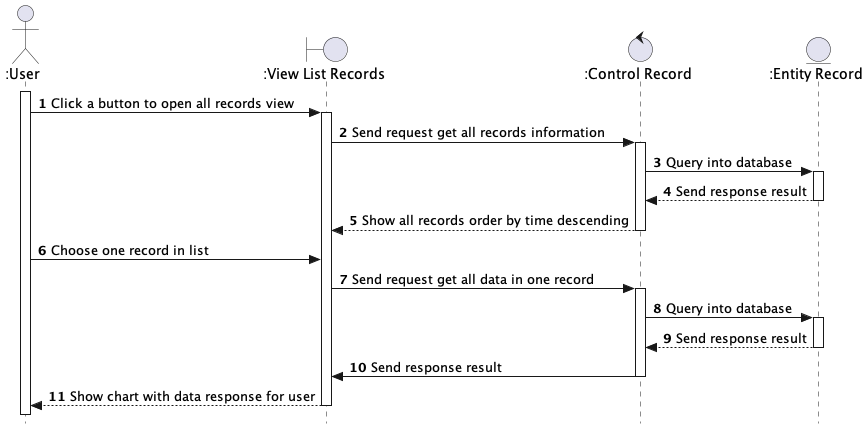
\includegraphics[width=16cm,height=11cm]{Images/mobile_app/view_record_timeline.png}
         \caption[Sơ đồ tuần tự chức năng xem lịch sử các lần đo trên App]{\bfseries \fontsize{12pt}{0pt}
         \selectfont Sơ đồ tuần tự chức năng xem lịch sử các lần đo trên App}
         \label{view_record_timeline} %đặt tên cho ảnh
    \end{figure}

    Sơ đồ tuần tự trên mô tả chi tiết quá trình người dùng xem lịch sử các lần đo. Người dùng chọn vào tab xem lịch sử, 
    lúc đó hệ thống sẽ gửi một yêu cầu lấy danh sách lịch sử các lần đo qua Control và hiển thị cho người dùng, sau đó người dùng sẽ
    chọn một bản ghi, Control sẽ lấy dữ liệu và hiển thị cho người dùng dữ liệu đo trên biểu đồ. Việc xử lý các yêu cầu cụ thể
    được chúng em thể hiện trong Hình \ref{} ở chương sau.

\paragraph{Sơ đồ tuần tự chức năng xem thay đổi thông tin cá nhân}
\mbox{}

  \begin{figure}[H]
        \centering
        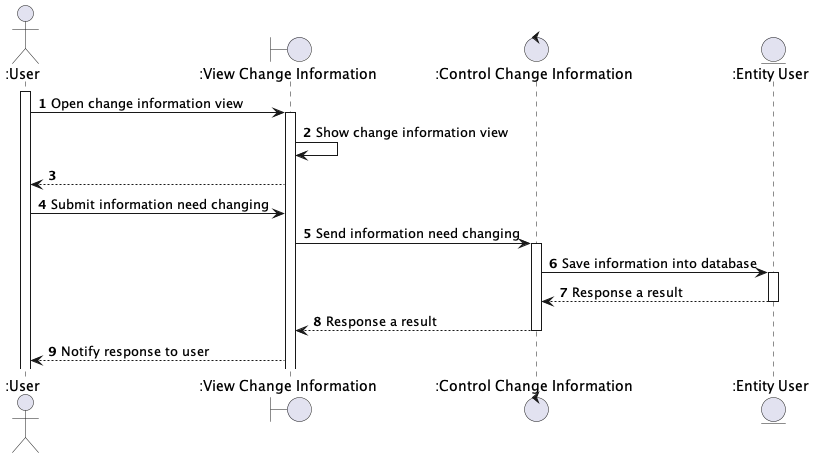
\includegraphics[width=16cm,height=11cm]{Images/mobile_app/change_user_information.png}
        \caption[Sơ đồ tuần tự chức năng xem thay đổi thông tin cá nhân trên App]{\bfseries \fontsize{12pt}{0pt}
        \selectfont Sơ đồ tuần tự chức năng xem thay đổi thông tin cá nhân trên App}
        \label{change_user_information} %đặt tên cho ảnh
  \end{figure}

  Sơ đồ tuần tự trên mô tả chi tiết quá trình người dùng thay đổi thông tin cá nhân. Người dùng thay đổi thông tin cá nhân
  và gửi yêu cầu. Control sẽ xử lý và lưu vào cơ sở dữ liệu, sau đó sẽ thông báo lại cho người dùng.
  Việc xử lý cụ thể như thế nào được chúng em thể hiện trong Hình \ref{} ở chương sau.

  \paragraph{Sơ đồ tuần tự chức năng đổi mật khẩu}
\mbox{}

  \begin{figure}[H]
        \centering
        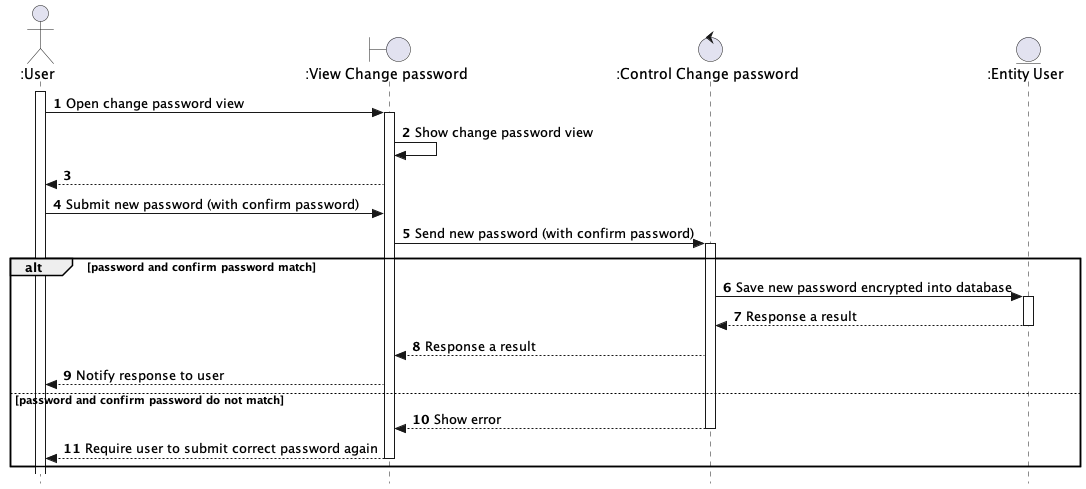
\includegraphics[width=16cm,height=11cm]{Images/mobile_app/change_password.png}
        \caption[Sơ đồ tuần tự chức năng đổi mật khẩu trên App]{\bfseries \fontsize{12pt}{0pt}
        \selectfont Sơ đồ tuần tự chức năng đổi mật khẩu trên App}
        \label{change_password} %đặt tên cho ảnh
  \end{figure}

  Sơ đồ tuần tự trên mô tả chi tiết quá trình người dùng đổi mật khẩu. Người dùng nhập mật khẩu và gửi yêu cầu đổi mật khẩu, 
  yêu cầu sẽ được xử lý bởi Control, nếu có lỗi phát sinh sẽ trả ra lỗi cho người dùng và yêu cầu người dùng nhập lại. Control
  sẽ xử lý cụ thể như thế nào được chúng em thể hiện trong Hình \ref{} trong chương sau.

\paragraph{Sơ đồ tuần tự chức năng xem/gửi tin nhắn}
\mbox{}

  \begin{figure}[H]
        \centering
        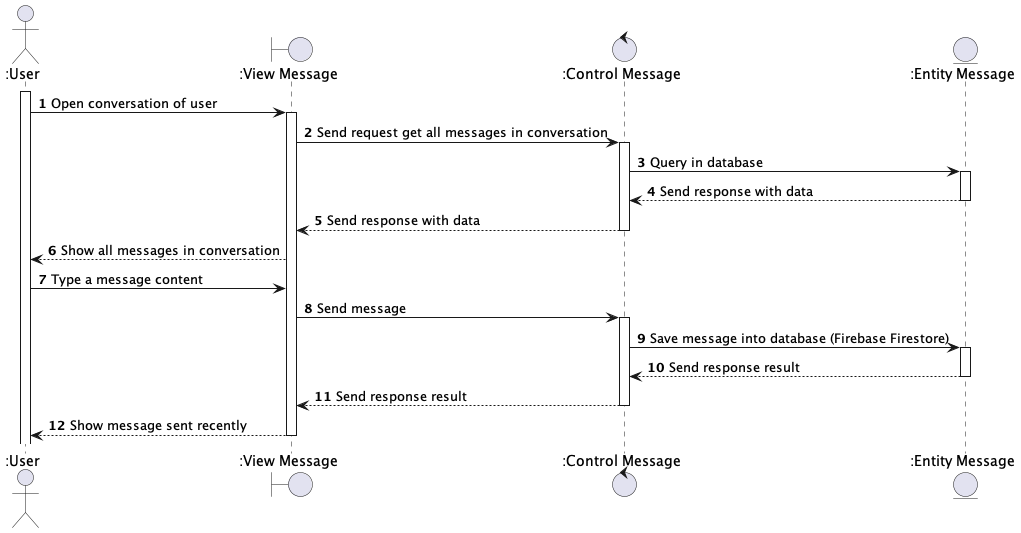
\includegraphics[width=16cm,height=11cm]{Images/mobile_app/send_and_receive_message.png}
        \caption[Sơ đồ tuần tự chức năng xem/gửi tin nhắn trên App]{\bfseries \fontsize{12pt}{0pt}
        \selectfont Sơ đồ tuần tự chức năng xem/gửi tin nhắn trên App}
        \label{send_and_receive_message} %đặt tên cho ảnh
  \end{figure}

  Sơ đồ tuần tự trên mô tả chi tiết quá trình người dùng xem và gửi tin nhắn. Người dùng click vào hội thoại để xem tin nhắn. 
  Nếu người dùng gửi tin nhắn, Control sẽ xử lý để gửi tin nhắn đến cho đối phương và lưu tin nhắn vào cơ sở dữ liệu, 
  chi tiết Control sẽ xử lý cụ thể như thế nào được chúng em thể hiện trong Hình \ref{} trong chương sau.


\paragraph{Sơ đồ tuần tự chức năng xem bài đăng tin tức}
\mbox{}

  \begin{figure}[H]
        \centering
        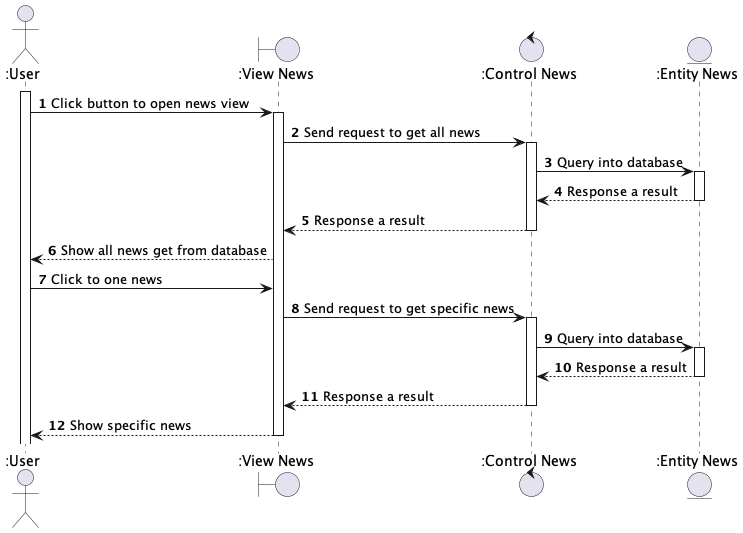
\includegraphics[width=16cm,height=11cm]{Images/mobile_app/view_news.png}
        \caption[ Sơ đồ tuần tự chức năng xem bài đăng tin tứctrên App]{\bfseries \fontsize{12pt}{0pt}
        \selectfont Sơ đồ tuần tự chức năng xem bài đăng tin tức trên App}
        \label{view_news} %đặt tên cho ảnh
  \end{figure}

  Sơ đồ tuần tự trên mô tả chi tiết quá trình người dùng xem tin tức/bài đăng. Người dùng chọn mở giao diện tin tức, API lấy tin tức sẽ
  được xử lý bởi Control, và hiện danh sách các bài đăng cho người dùng, sau đó người dùng chọn một bài đăng thì thông tin chi tiết
  của bài đăng sẽ hiển thị cho người dùng. Cụ thể về việc xử lý các yêu cầu của Control được chúng em thể hiện trong Hình \ref{} trong chương sau.

\paragraph{Sơ đồ tuần tự chức năng bật/tắt Bluetooth}
\mbox{}

  \begin{figure}[H]
        \centering
        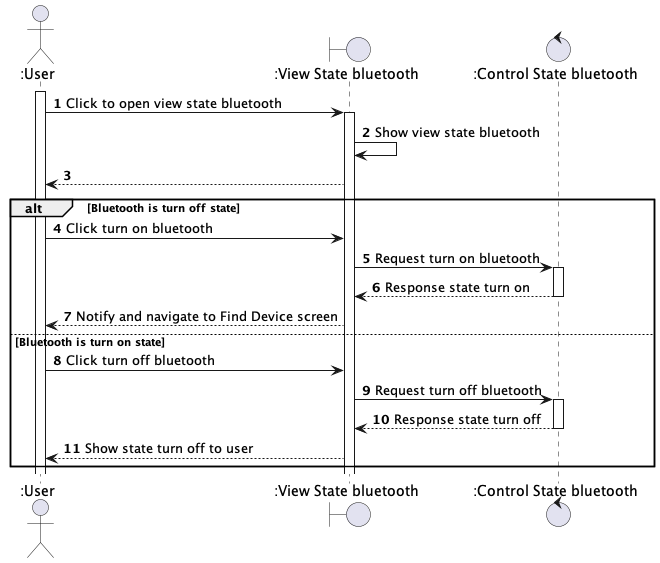
\includegraphics[width=16cm,height=12cm]{Images/mobile_app/turn_on_off_bluetooth.png}
        \caption[Sơ đồ tuần tự chức năng bật/tắt Bluetooth trên App]{\bfseries \fontsize{12pt}{0pt}
        \selectfont Sơ đồ tuần tự chức năng bật/tắt Bluetooth trên App}
        \label{turn_on_off_bluetooth} %đặt tên cho ảnh
  \end{figure}

  Sơ đồ tuần tự trên mô tả chi tiết quá trình bật/tắt Bluetooth. Người dùng gửi yêu cầu bật hoặc tắt Bluetooth, Control sẽ kiểm tra
  trạng thái Bluetooth và truy cập vào phần cứng thực hiện yêu cầu của người dùng.

\paragraph{Sơ đồ tuần tự chức năng kết nối Bluetooth với thiết bị đo điện tim}
\mbox{}

  \begin{figure}[H]
        \centering
        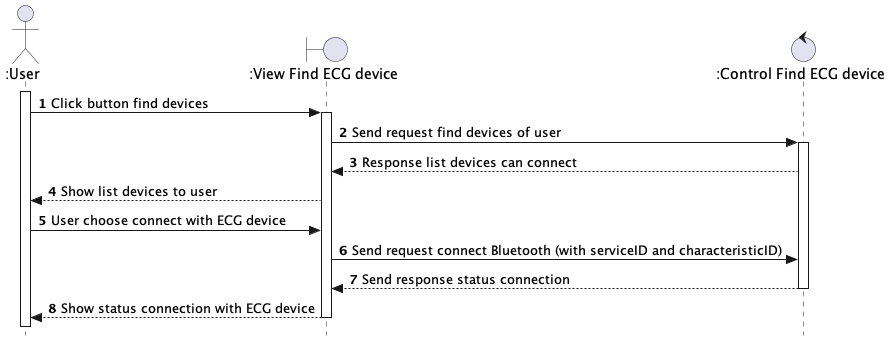
\includegraphics[width=16cm,height=10cm]{Images/mobile_app/connect_with_device.png}
        \caption[Sơ đồ tuần tự chức năng kết nối Bluetooth với thiết bị đo điện tim trên App]{\bfseries \fontsize{12pt}{0pt}
        \selectfont Sơ đồ tuần tự chức năng kết nối Bluetooth với thiết bị đo điện tim trên App}
        \label{connect_with_device} %đặt tên cho ảnh
  \end{figure}

  Sơ đồ tuần tự trên mô tả chi tiết quá trình người dùng kết nối với thiết bị đo điện tim. Người dùng sau khi bật Bluetooth
  sẽ có thể tìm kiếm thiết bị và xem các danh sách các thiết bị mình tìm thấy. Người dùng chọn đúng thiết bị (theo tên) 
  và thực hiện kết nối, kết quả của việc kết nối sẽ được hiện trên màn hình.

\paragraph{Sơ đồ tuần tự chức năng ngắt kết nối Bluetooth với thiết bị đo điện tim}
\mbox{}

  \begin{figure}[H]
        \centering
        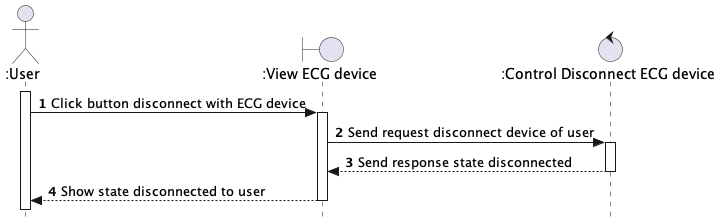
\includegraphics[width=16cm,height=9cm]{Images/mobile_app/disconnect_with_device.png}
        \caption[Sơ đồ tuần tự chức năng ngắt kết nối Bluetooth với thiết bị đo điện tim trên App]{\bfseries \fontsize{12pt}{0pt}
        \selectfont Sơ đồ tuần tự chức năng ngắt kết nối Bluetooth với thiết bị đo điện tim trên App}
        \label{disconnect_with_device} %đặt tên cho ảnh
  \end{figure}

  Sơ đồ tuần tự trên mô tả chi tiết quá trình người dùng ngắt kết nối với thiết bị đo điện tim. Trong khi đang kết nối, người dùng
  có thể chọn ngắt kết nối Bluetooth giữa thiết bị và ứng dụng, sau khi ngắt kết nối, sẽ có thông báo
  hiển thị trên màn hình.

\paragraph{Sơ đồ tuần tự chức năng tiến hành đo điện tim}
\mbox{}

  \begin{figure}[H]
        \centering
        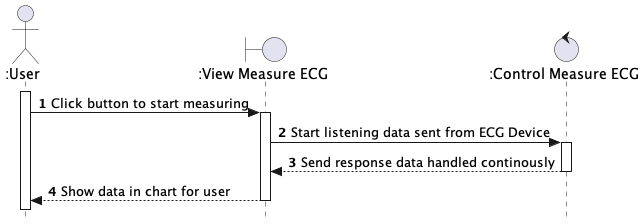
\includegraphics[width=16cm,height=9cm]{Images/mobile_app/start_measuring_ecg.png}
        \caption[Sơ đồ tuần tự chức năng tiến hành đo điện tim trên App]{\bfseries \fontsize{12pt}{0pt}
        \selectfont Sơ đồ tuần tự chức năng tiến hành đo điện tim trên App}
        \label{start_measuring_ecg} %đặt tên cho ảnh
  \end{figure}
 
  Sơ đồ tuần tự trên mô tả chi tiết quá trình người dùng bắt đầu quá trình đo điện tim. Để bắt đầu được quá trình đo, điều
  kiện đó là người dùng đã kết nối thiết bị với ứng dụng để có thể lắng nghe được dữ liệu từ Bluetooth trả ra. Sau khi nhấn nút bắt đầu đo,
  dữ liệu lắng nghe sẽ được xử lý và thể hiện trên biểu đồ cho người dùng.

\paragraph{Sơ đồ tuần tự chức năng kết thúc quá trình đo điện tim}
\mbox{}

  \begin{figure}[H]
        \centering
        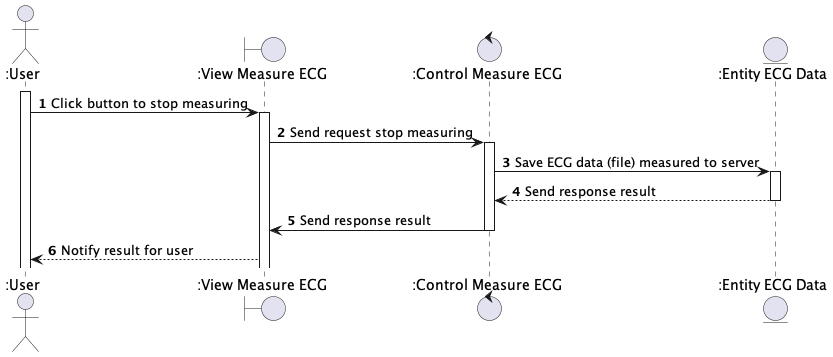
\includegraphics[width=16cm,height=9cm]{Images/mobile_app/end_measuring_ecg.png}
        \caption[Sơ đồ tuần tự chức năng kết thúc quá trình đo điện tim trên App]{\bfseries \fontsize{12pt}{0pt}
        \selectfont Sơ đồ tuần tự chức năng kết thúc quá trình đo điện tim trên App}
        \label{end_measuring_ecg} %đặt tên cho ảnh
  \end{figure}

  Sơ đồ tuần tự trên mô tả chi tiết quá trình người dùng kết thúc quá trình đo điện tim. Trong khi đang đo, nếu người dùng muốn dừng, 
  việc kết thúc quá trình đo đồng nghĩa với dữ liệu đo được lưu lên cơ sở dữ liệu để bác sĩ có thể theo dõi.
\newpage
